The combination of the components used in an experiment, their properties, their position, etc amounts to what we call the \textit{experiment configuration}. Experiment configurations vary depending on the nature of the experiment. A precise description of this configuration is vital if we are to analyse our results reliably, hence the need for a file format that is appropriate for capturing all of this information.

\begin{wrapfigure}{L}{0.5\linewidth}
\begin{center}
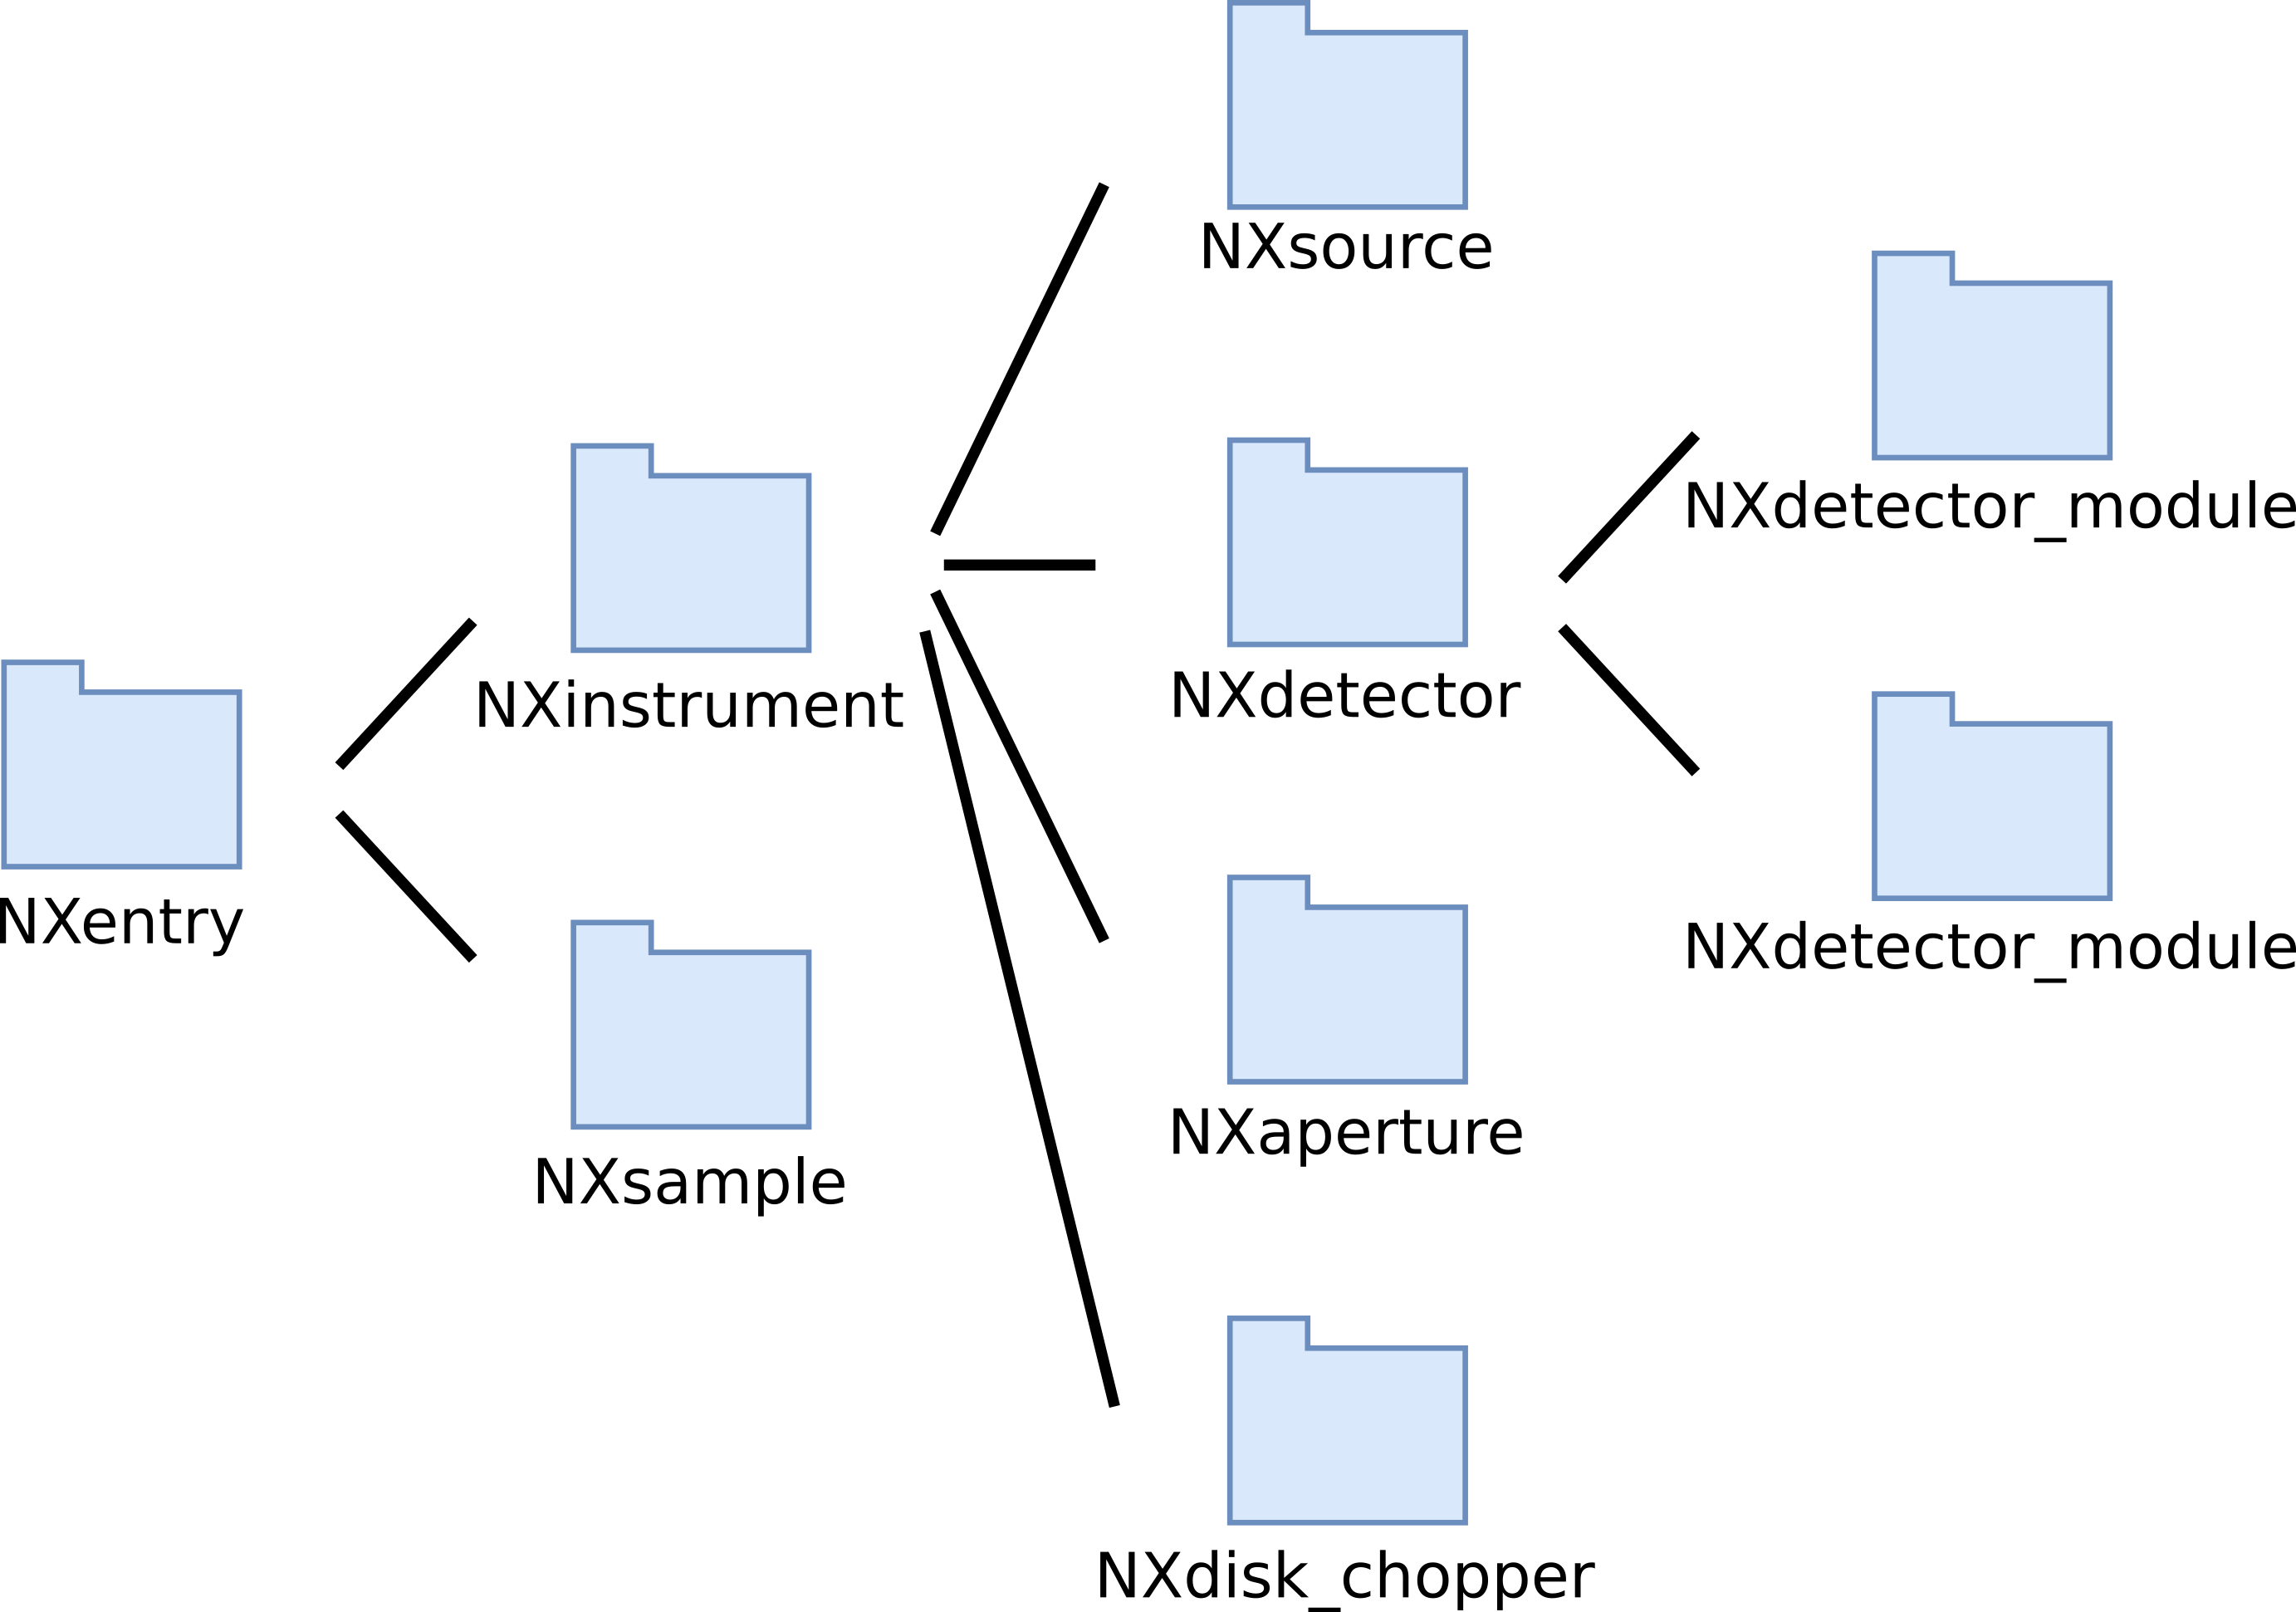
\includegraphics[width=0.8\linewidth]{instrument_arch.png}
\end{center}
\caption{A typical NeXus file layout}
\vspace{-50pt}
\end{wrapfigure}

The NeXus file format was developed with the aim of:
\begin{itemize}
\item Creating a file format which is common to different neutron facilities.
\item Storing all experiment data in a single file.
\item Allowing experiment data to be loaded into a variety of different software tools without the need for conversion.
\end{itemize}
\smallskip
NeXus is built on top of the HDF5 file format. It adds domain-specific rules for organising data and has a dictionary of well-defined domain-specific field names pertaining to the components used in neutron experiments and their characteristics. The \texttt{pandas} library also offers an interface for HDF5 files.
